\documentclass{article}

\usepackage{enumitem}
\usepackage{amsmath}
\usepackage{amsfonts}
\usepackage{amssymb}
\usepackage[margin=0.5in]{geometry}
\usepackage[hidelinks, bookmarks=false]{hyperref}

\usepackage[dvipsnames]{xcolor}

\let\oldemptyset\emptyset
\let\emptyset\varnothing
\newcommand{\R}{\mathbb{R}}
\newcommand{\Rd}{\R^d}

\usepackage{environ}
\NewEnviron{centerframebox}{\begin{center}\fbox{\parbox{0.92\textwidth}{\BODY}}\end{center}}

\title{Discrete and Computational Geometry \\ Assignment 7}
\author{
  \AA{AAAAAAAAAA AAAAAAA}{6} \\
  \href{mailto:\AA{AAAAAAAAAAAAAAAAAAAA}{7}}{\AA{AAAAAAAAAAAAAAAAAAAA}{7}}
  \and
  Emilia Groß-Hardt \\
  \href{mailto:emilia.ghdt@uni-bonn.de}{emilia.ghdt@uni-bonn.de}
}

\usepackage{graphicx}
\graphicspath{{./} {img/}}

\usepackage{titlesec}
\titleformat{\section}
  {\normalfont\Large\bfseries}{Problem \thesection : }
  {0em}{\mdseries}

\date{December 6, 2024}

\begin{document}
  \maketitle
  \begin{center}
    { \bfseries Deadline: 6 Dec 2024, 23:55 }
  \end{center}

  \section{}
  \subsection{(a)}
  TODO

  \subsection{(b)}
  The NW chains of faces have, on average, the same complexity as the faces themselves by a factor of $\frac14$.
  So if we show that the sum of the NW chains in the zone of $l$ has complexity $O(n)$,
  then the complexity of the zone will also be $O(n)$.
  Let's define the concept of a \textit{short NW chain} (SNW) as the NW chain, excluding its topmost edge.
  The order of its complexity will also be the same as the complexity of the face.

  Using statement (a), any line in $L$ that contributes to a SNW chain can only do so for one face.
  So the sum of the lengths of SNW chains in the zone of $l$ is limited by the number of lines in $L$.
  Thus, it has order $O(n)$, and the zone complexity of $l$ also has order $O(n)$.

  \section{}
  \begin{centerframebox}
    Consider the example of the 5 points. Draw the Voronoi diagram
    of order $k = 2$. Which subsets of points have a non-empty Voronoi region?
  \end{centerframebox}
  The Voronoi diagram features 7 regions.
  Corresponding to the pairs:
  \[(p_1,p_2),\, (p_1,p_3),\, (p_1,p_4),\, (p_2,p_4),\, (p_2,p_5),\, (p_3,p_4),\, (p_4,p_5)\]

  \begin{center}
    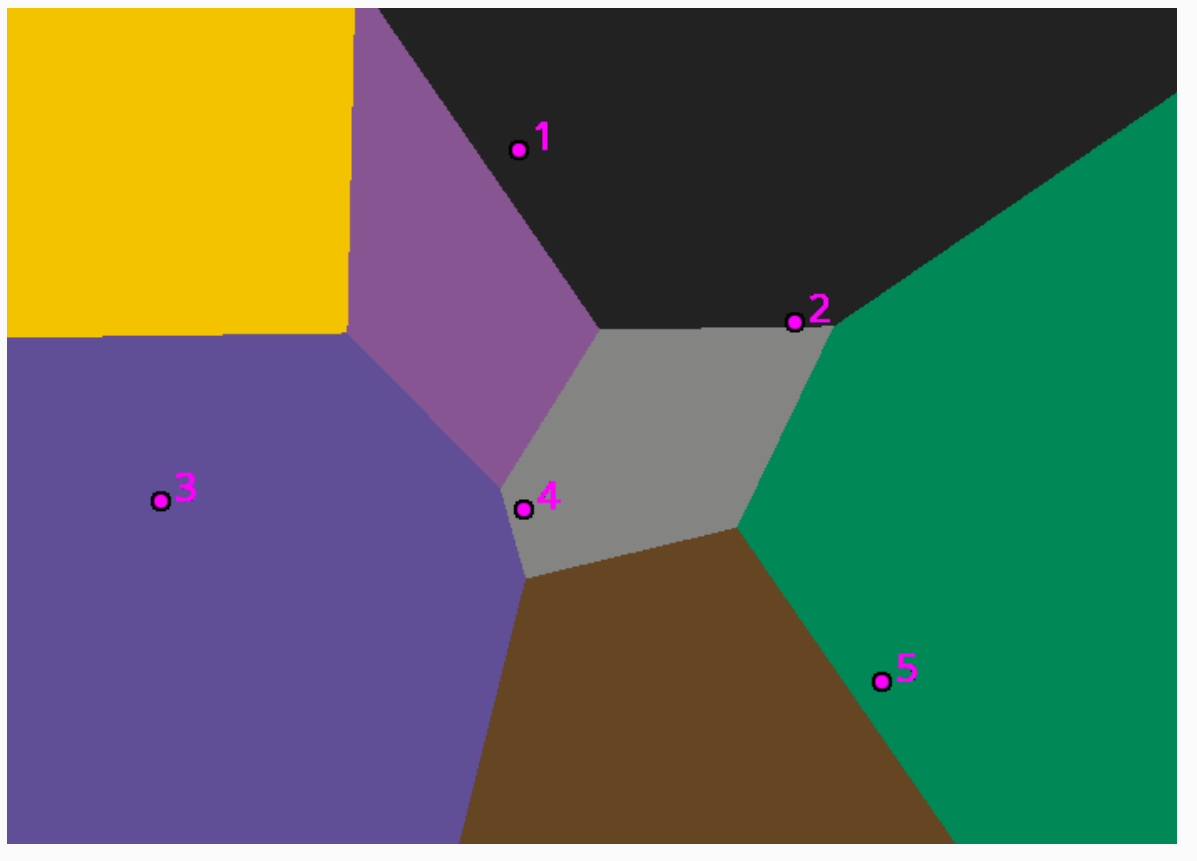
\includegraphics[width=.7\textwidth]{order-2}

    Figure 1: The order $k=2$ Voronoi diagram
  \end{center}
  % (c) Clover

  \section{}
  \begin{centerframebox}
    Let $P$ be a set of $n$ points in the plane in general position (no three points on a line, no four
    points on a circle). Show that the graph of the order-$(n - 1)$ Voronoi diagram of $P$ has $O(n)$
    Voronoi vertices and Voronoi edges.
  \end{centerframebox}
  Since the order is one less than the number of points,
  this is equivalent to finding which point is the farthest away one,
  as apposed to finding the $n-1$ nearest neighbors.

  This way each region of the Voronoi diagram corresponds to one point in $P$, so there are $O(n)$ regions.
  There's a proof%
  \footnote{\href{https://www.cs.purdue.edu/homes/cs53100/slides/voronoi.pdf\#Navigation7}{
    Voronoi Diagrams (chapter 7) -- Elisha Sacks. Purdue University
  }}
  that a regular Voronoi diagram has $O(n)$ edges and vertices,
  that only uses the fact that it is a planer graph (if we connect the point at infinity)
  and that it has no vertices connected to only two edges.
  Which both holds for our $n-1$ order diagram as well.
  % (c) Clover

\end{document}
